%% LyX 1.6.5 created this file.  For more info, see http://www.lyx.org/.
%% Do not edit unless you really know what you are doing.
\documentclass[english]{article}
\usepackage[T1]{fontenc}
\usepackage[latin9]{inputenc}
\usepackage{graphicx}

\usepackage[letterpaper]{geometry}
\usepackage{listings}
\geometry{verbose,tmargin=2.5cm,bmargin=2.5cm,lmargin=2.5cm,rmargin=2.5cm}

\usepackage[final]{pdfpages} % For including extra pages.


\usepackage{listings}
\lstset{ language=VHDL }   % For code blocks
\makeatletter

%%%%%%%%%%%%%%%%%%%%%%%%%%%%%% LyX specific LaTeX commands.
%% Because html converters don't know tabularnewline
\providecommand{\tabularnewline}{\\}

\makeatother

\usepackage{babel}

% The following can be used if not using custom frontpage
\title{<document title>}
\author{<name>\\
        \\
        <student id>
}
\date{\today}



\begin{document}
%\includepdf{frontpage.pdf}
\begin{titlingpage}
\centering \parindent=0pt
\newcommand{\HRule}{\rule{\textwidth}{1mm}}
\vspace*{\stretch{1}} \HRule\\[1cm]\Huge\bfseries
Internship report\\[0.7cm]
\large Atkins Denmark\\[1cm]
\HRule\\[4cm]  
\large by Kim Rostgaard Christensen, s084283\\
\vspace*{\stretch{2}} \normalsize %
\begin{flushleft}
Technical University of Denmark\\
Institute for Mathematical Modelling\\
Internship at Atkins Denmark\\
Per Stoltze\\
\today \end{flushleft}
\end{titlingpage}


\begin{abstract}
 \begin{abstract}
This report document my three-months internship with Atkins Denmark. The internship is part of my education, and is reduced from 20 weeks to 3 months due to received merits.
\end{abstract}

\end{abstract}

\tableofcontents
\newpage

\section{Project description}
\label{sec:project_description}
The main requirements of the Vending Machine (VM):

\begin{enumerate}
\item The VM can sell one product, a coke-can.
\item When a sufficient amount of coins is inserted, one cocke-can will be dispensed from the VM.
\item The products price is fixed to 7 kr. ( in design this should be changeble )
\item The VM accepts 1 and 2 Kr coins.
\item A display should show the current total amount of money inserted.
\item A LED should indicate if change is avaliable (min 1 kr coin available).
\item Remove product sensor, will close the the coin slot and turn on indicating LED until product is removed.
\item Return Change.
\item Return all Coins.
\item If change is not available, the machine should only accept purchases with the right amount.
\end{enumerate}

% 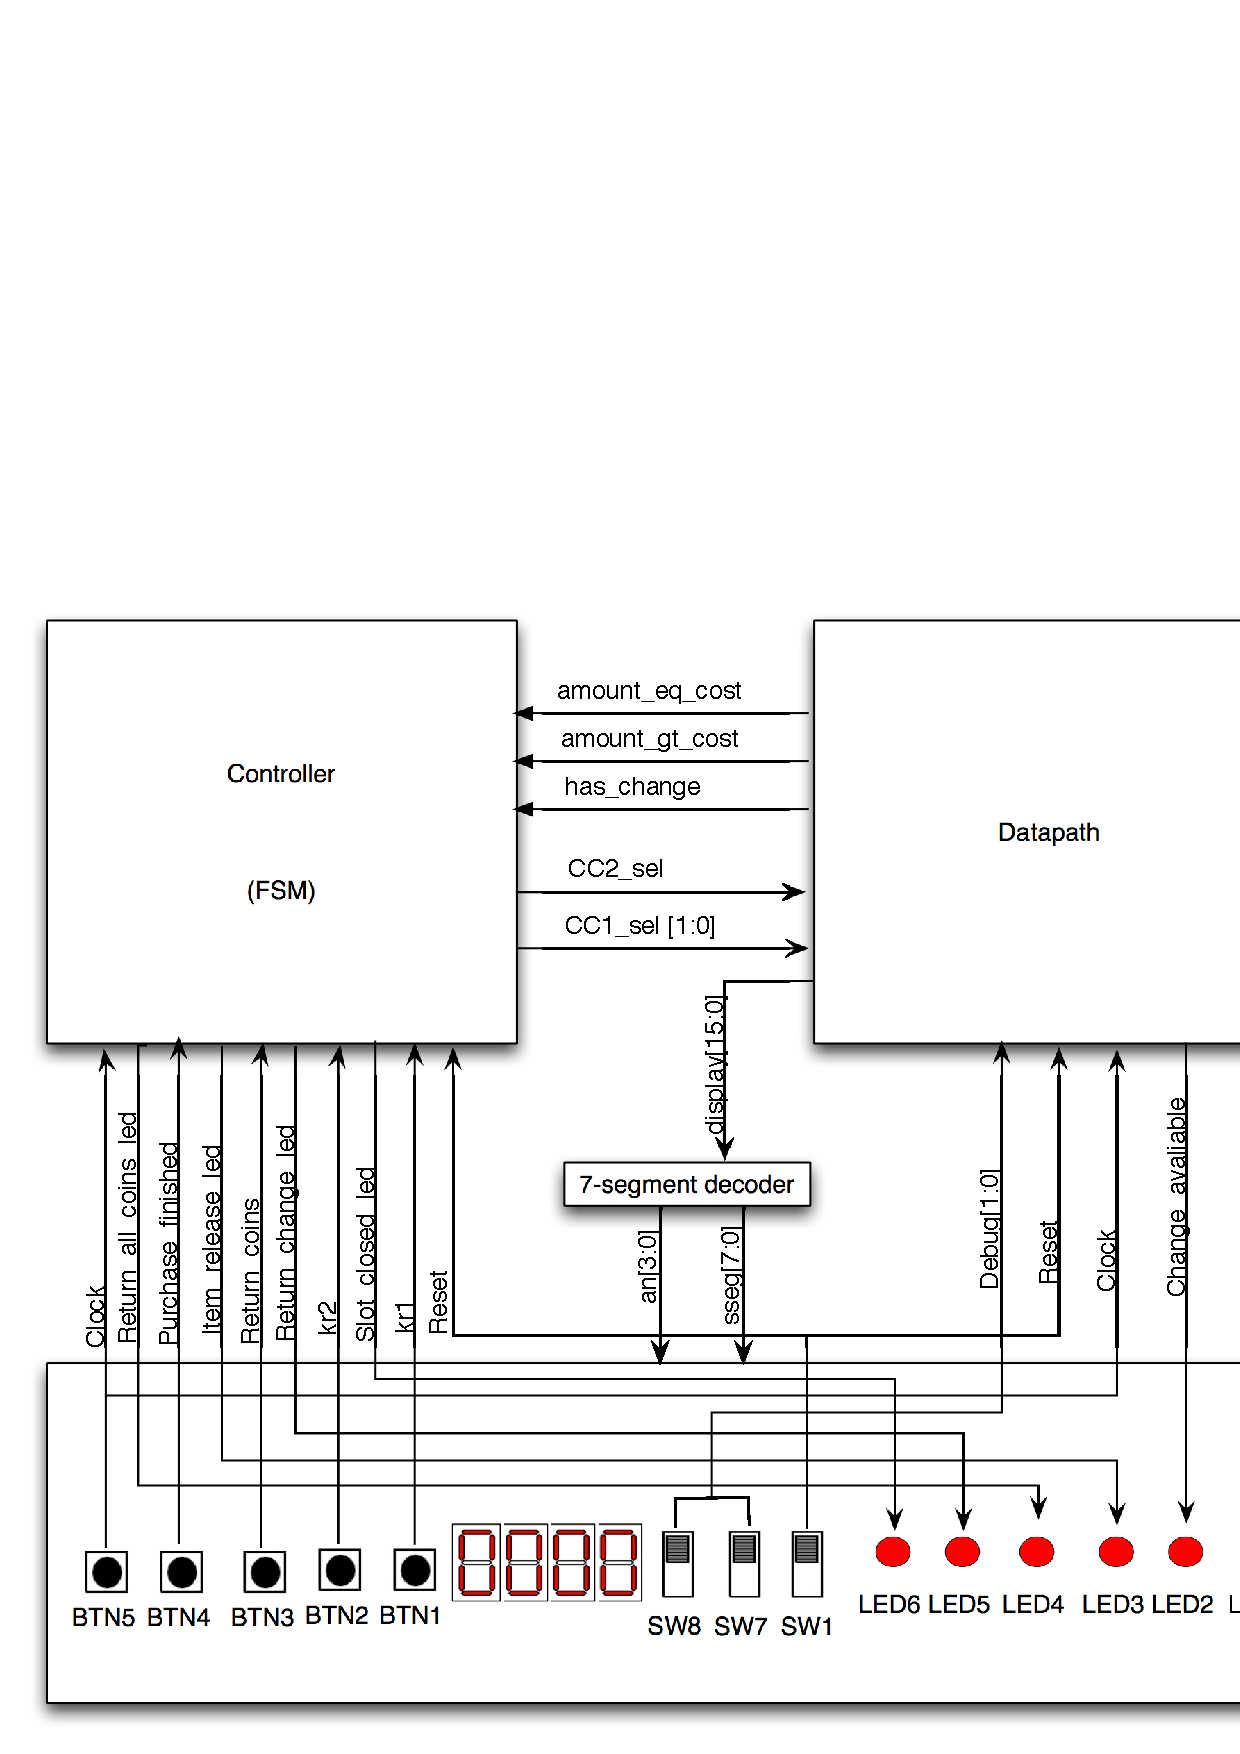
\includegraphics[scale=0.75]{fig/SystemDescription.png}


\section{Specification analysis}
By studying the specification we conclude that we will be needing
eight different states; one for each {}``circle''. For input we
need a control for the direction (clockwise or counter-clockwise)
and a reset switch.

For output we would at minimum need to specify the orientation and
the number of the current circle to be displayed. These are defined
as top,d1,d0 (d for digit).\\
\\
Following the specification flow, leaves us with the following
finite state machine.

\begin{figure}[!htbp] 
	\centering 
        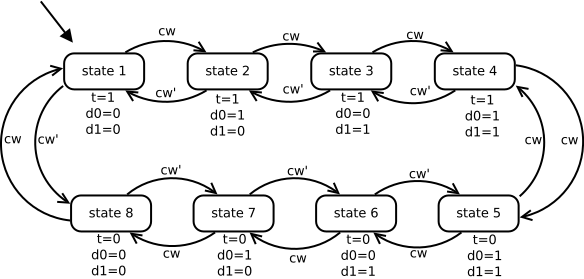
\includegraphics[width=0.7\textwidth]{fig/FSM_states.pdf}
	\caption{States of our circiut}
	\label{fig:states} 
\end{figure}


\begin{figure}[!htbp] 
	\centering 
        \includegraphics[width=0.5\textwidth]{fig/Block_diagram.pdf}
	\caption{Block diagram}
	\label{fig:block_diagram} 
\end{figure}


\section{Solution description}
\label{sec:solutions_description}
For our solution we tried to do a 1:1 mapping directly from drawings to VHDL. This means that each ``box'' in our design
became a VHDL module. This lead to the three following files: ``Runner_logic.vhd'',``Runner_Registry.vhd'',``Runner.vhd''


\subsection{Implementation}
\begin{figure}[!htbp] 
	\centering 
        \includegraphics[height=0.4\textwidth]{fig/Block_diagram_implementation.pdf}
	\caption{Block diagram of implementation}
	\label{fig:block_diagram} 
\end{figure}
For making this implementation we have created two new VHDL modules: ``sseg_decoder.vhd'' and ``clockscaler.vhd''. The clockscaler does a downscaling by a factor $10^{6}$ effectively setting the frequency to 5Hz (when having a period of 20ns).\\
The seven segment decoder translates inputs to the physical display.

\subsection{RTL level design}
The RTL level design was created using two muxes instead of combinatorial circuits. The code can be found in ``RTL/Runner_logic.vhd''.

\section{Development process}
\label{sec:development_process}
A software development process is the structure needed to development any type of software products. 
There are several models for such development processes, each describing differed approaches to get the software developed.

\subsection{Software Development Models}
Many of the larger scale models such as Unified Process, Waterfall, Scrum or Spiral Model isn't suitable for small projects  of  4 weeks. But on the other hand Models like eXtreme Programming haven't got the diagrams and design phases needed for our learning curve of VHDL. The model we used was a mix of the differed models that had all the phases and methods we needed.

\subsection{Planning phase}
In this phase we read the assignment, analyze the requirements and go over the inputs, outputs and hints.
Then we made the first version of our High Level State Machine and.

\subsection{Implementation phase}
With the information from planning we started programming the VM. During this process we made our Data path diagram and several updates to the State Diagram.

\subsection{Testing phase}
In the Testing Phase all our test benches has been made to find the last few bugs and errors. 

\subsection{Documenting phase}
In the Documenting phase we had all the information needed. A working product, a lot of diagrams, and many test cases. We wrote our documentation in \LaTeXe  because it focuses more on documentation that typesetting and it makes managing and maintaining larger papers easier.

\section{Tests}
%During development of the circiut, we did out testing via a number of VHDL testbenches. These were used to assert that our 
develeopment went in the right direction, and also to verify that the indivudial circuits worked as planned.
\subsection{Testbenches}
During development we used three major testbenches. One for the combinatorial circuit, one for the register, and one for the 
two put together.



\section{Conclusion}
\chapter{Conclusion}
\label{chap:conclusion}
In the beginning of the project we spent a great deal of time cleaning and refactoring code, making it more modulary and easy to navigate. But as the application evolved and grew in size and complexity, it became increasingly difficult to maintain a consistency in the code. Espeacially when thing were not doing as planned. New code arose in places where it did not belong.\\
From this we have learned about the importance of defining a clear program structure and functionality from the start of the project, and enforcing it thoughout the development process.\\\\
The webserver is responding slowly, but is very functional. The xsl transformations works like a charm in modern browsers and should definitly be considered in the case of an official http+xml implementation.\\\\
The LCD screen, acting as both in- an output, gives a quick way of getting an overview of the current status of the system. As well as modifying the system paramters realtime.\\ The values displayed are a bit off, due to programming errors. But it gives you an idea on how a finished system should look and behave.


\newpage
\appendix
\section{Timetable}
\begin{tabular}{c|c|c|c|c|c|c|c}
Date & Individual & Design & Implementation & Test & Documentation & Other & Total\tabularnewline
\hline
\hline 
03/05/2010 & MHI & 6 &  &  &  &  & 6\tabularnewline
\hline 
03/05/2010 & KRC & 6 &  &  &  &  & 6\tabularnewline
\hline 
03/12/2010 & MHI &  & 4 &  &  &  & 4\tabularnewline
\hline 
03/12/2010 & KRC &  & 8 &  &  &  & 8\tabularnewline
\hline 
03/19/2010 & MHI &  &  & 6 &  &  & 6\tabularnewline
\hline 
03/19/2010 & KRC &  &  & 6 &  &  & 6\tabularnewline
\hline 
03/23/2010 & MHI &  &  &  & 8 &  & 8\tabularnewline
\hline 
03/23/2010 & KRC &  &  &  & 8 &  & 8\tabularnewline
\hline
\hline 
 & Total & 12 & 12 & 12 & 16 & 0 & 52\tabularnewline
\cline{2-8} 
\end{tabular}

\section{Report distribution}
Kim Rostgaard Christensen (KRC)
\begin{itemize}
\item Sections \ref{sec:solutions_description} and \ref{sec:requirement_analysis}
\item Figures \ref{fig:fsm}, \ref{fig:fsmd}, \ref{fig:datapath} and \ref{fig:debug}
\end{itemize}

Morten Hillebo (MHI) 
\begin{itemize}
\item Sections \ref{sec:project_description}
\end{itemize}


\section{Figures}
\label{app:figures}


\begin{figure}
\centering
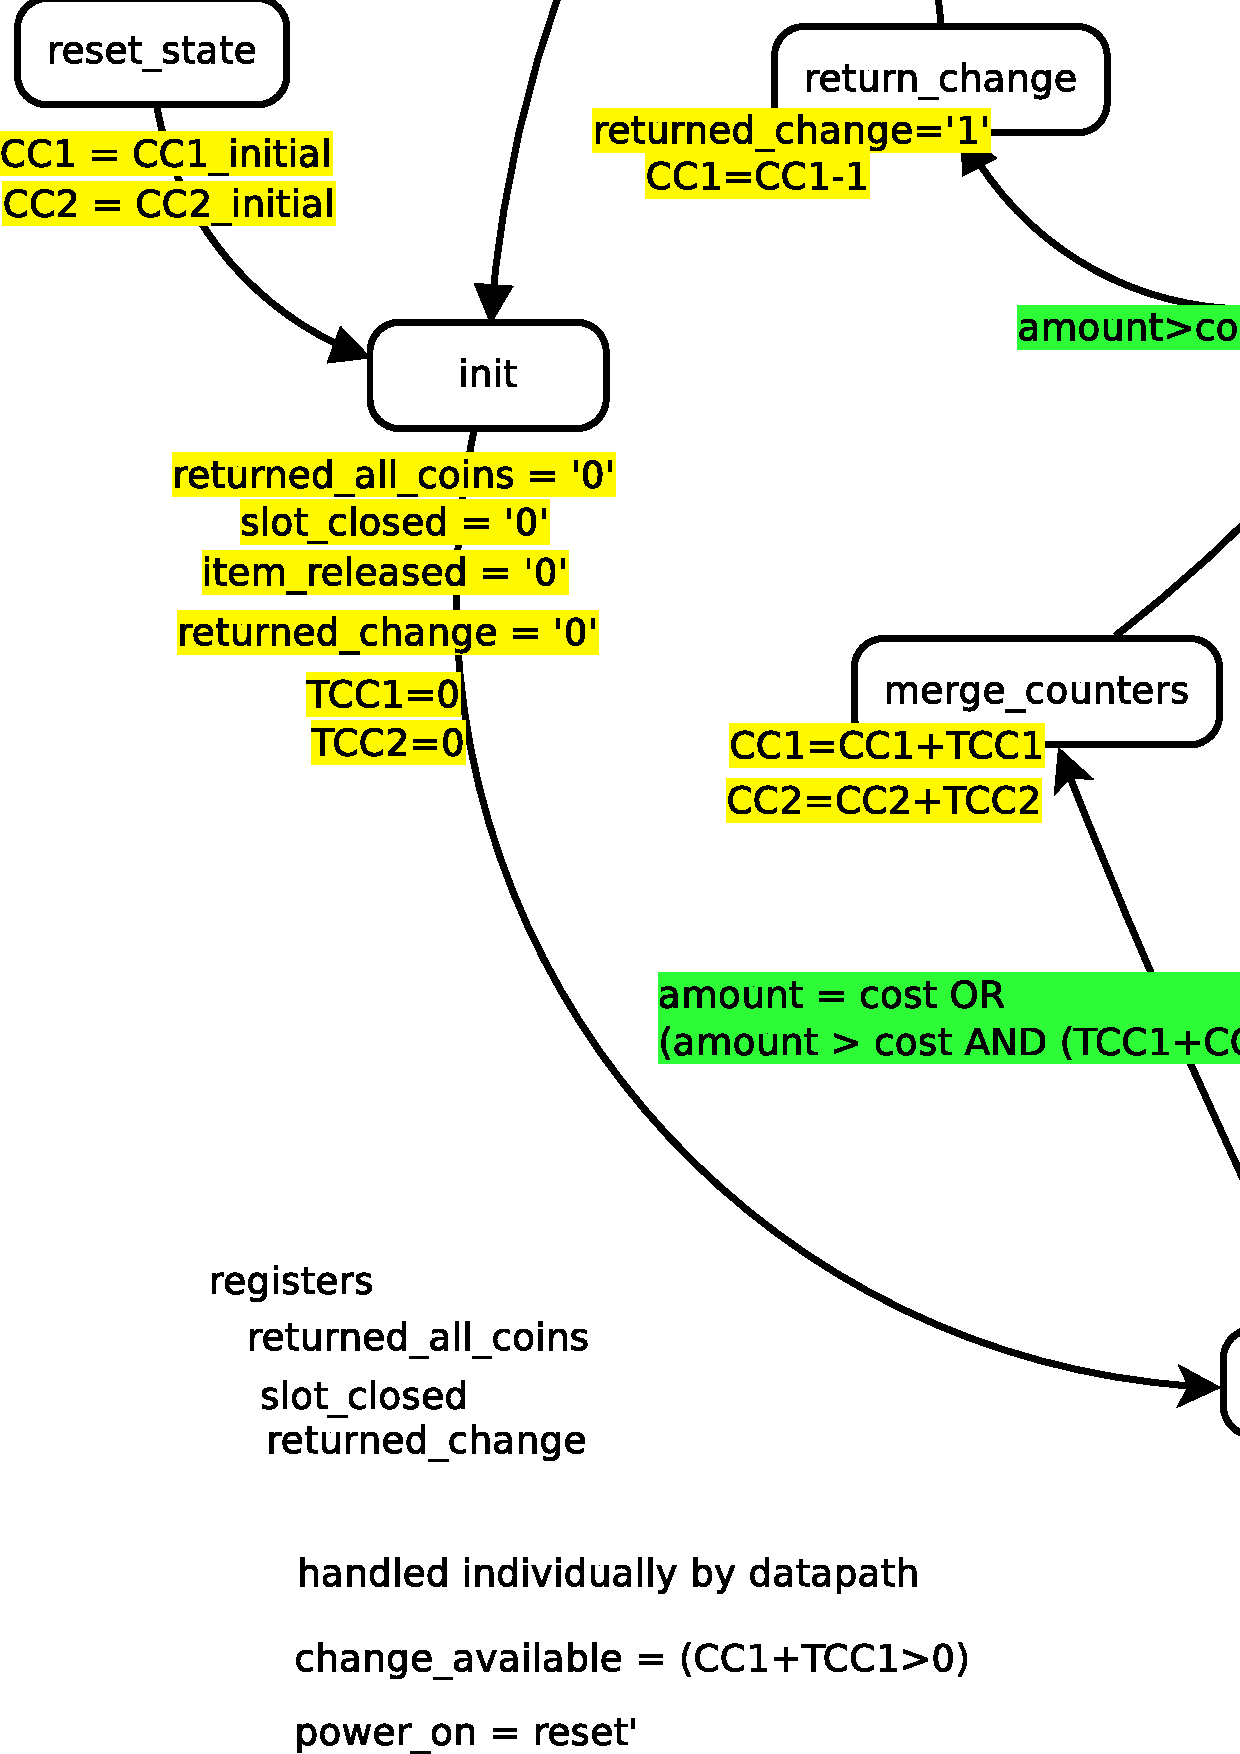
\includegraphics[width=1.0\textwidth]{fig/FSMD.pdf}
\caption{Finite statemachine with data}
\label{fig:fsmd}
\end{figure}

\begin{figure}
\centering
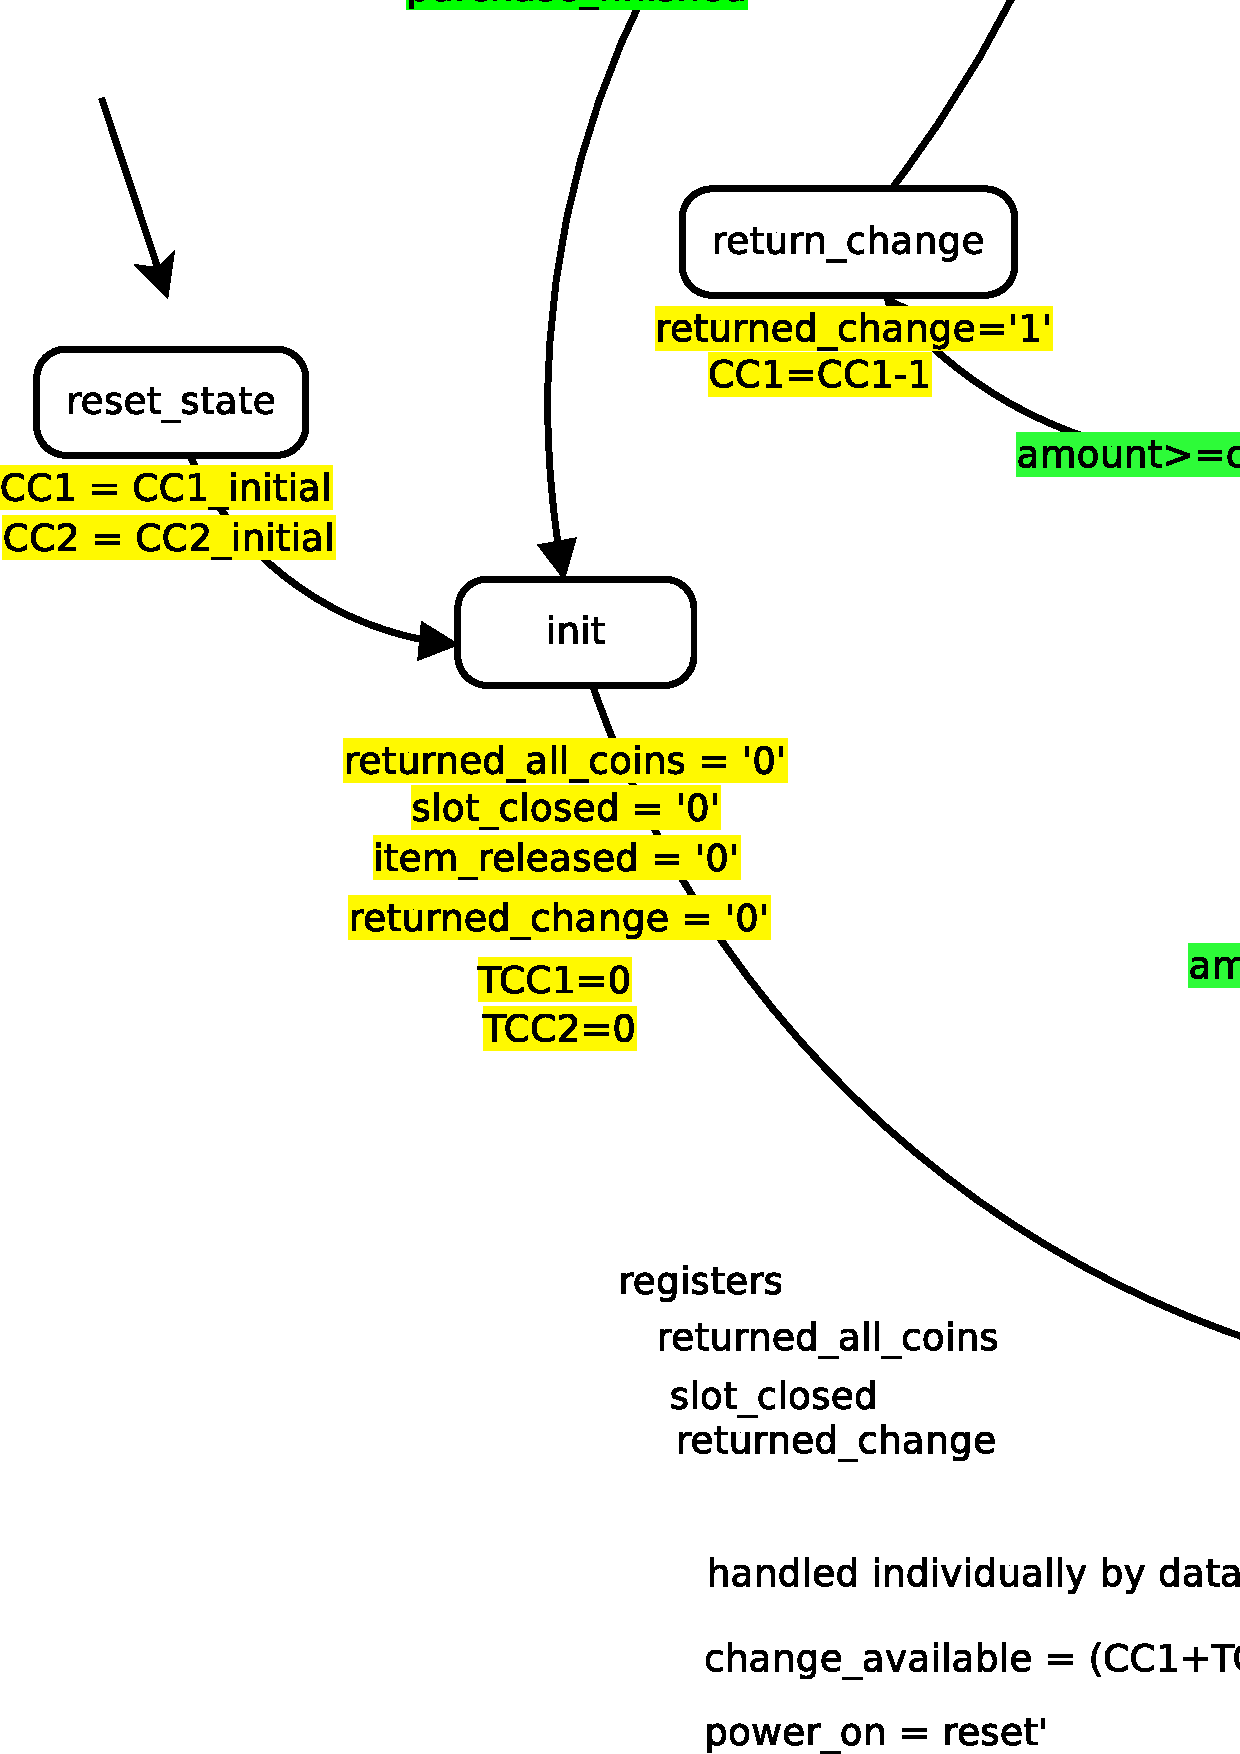
\includegraphics[width=1.0\textwidth]{fig/FSM.pdf}
\caption{Finite statemachine}
\label{fig:fsm}
\end{figure}

\begin{figure}
\centering
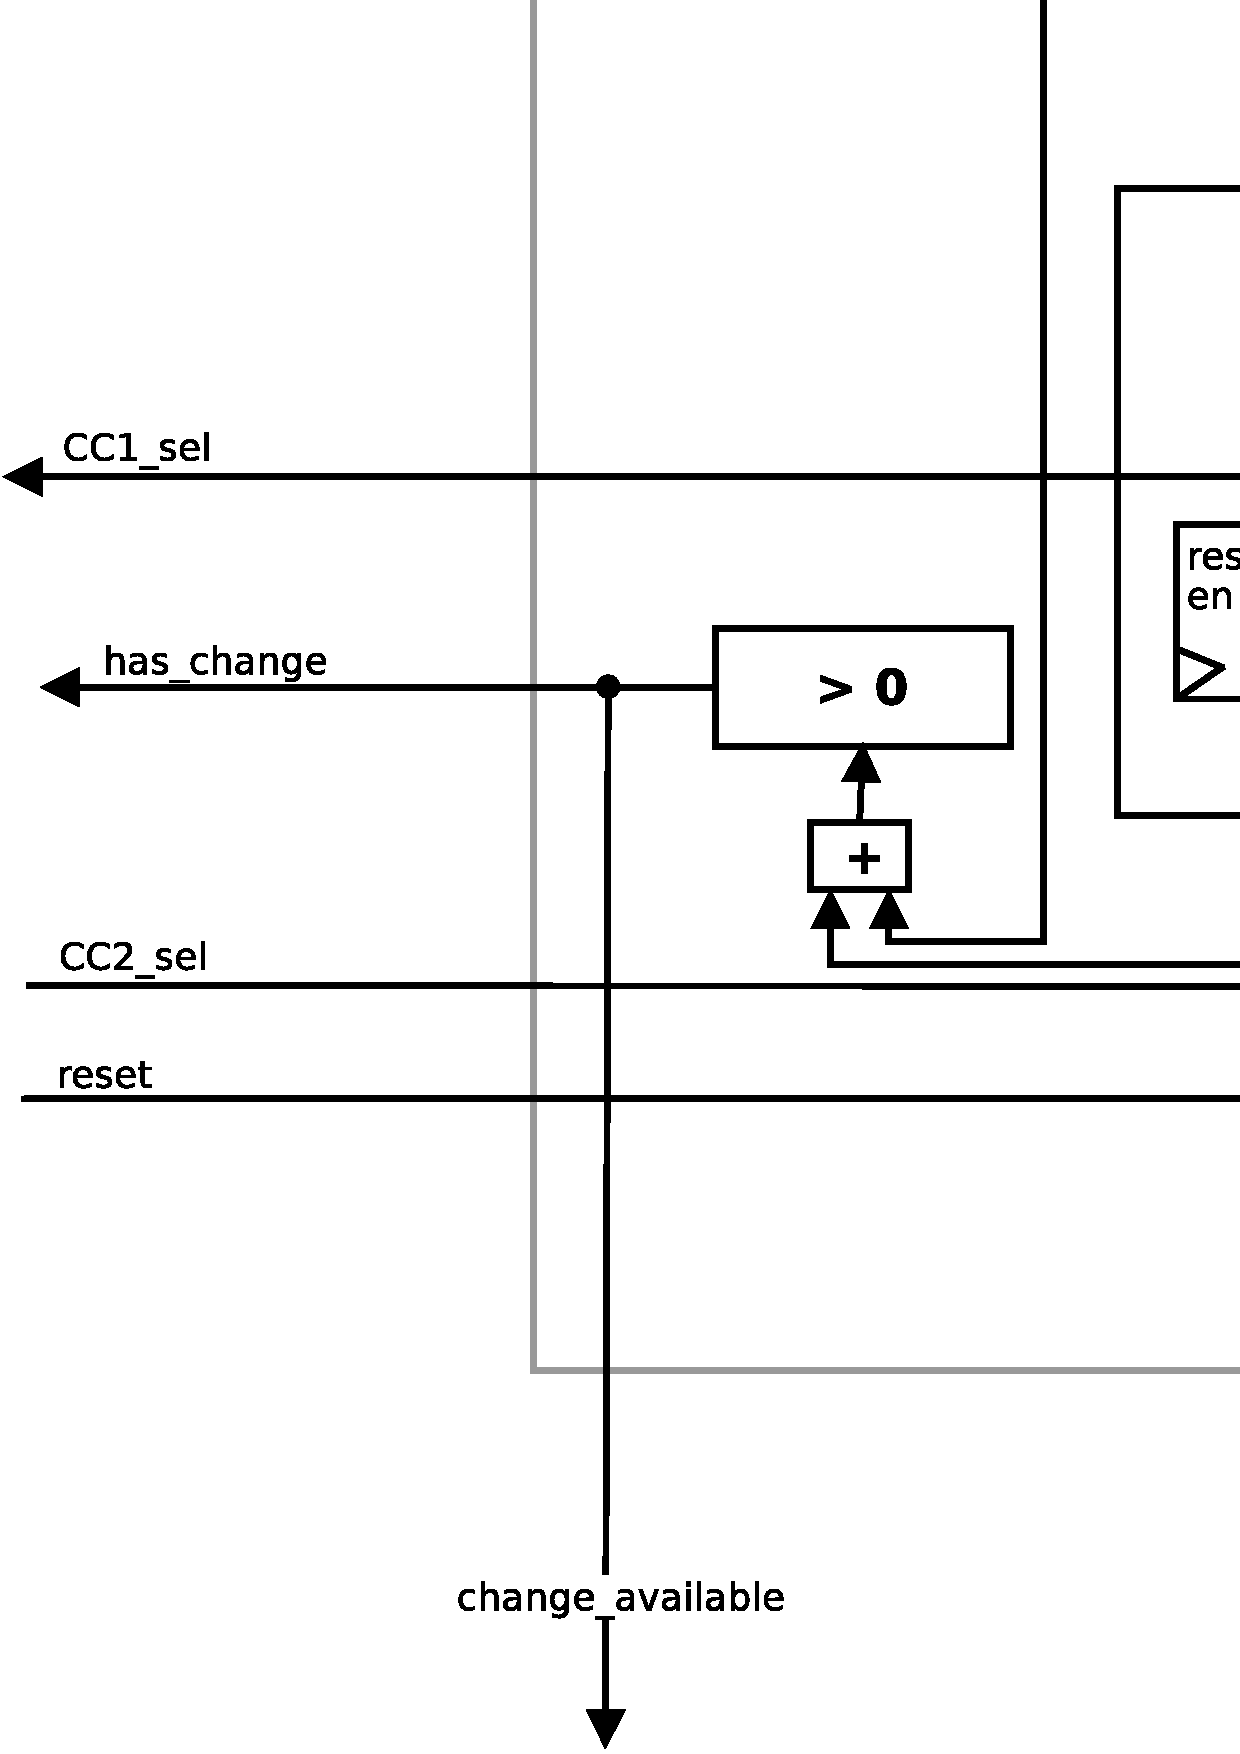
\includegraphics[width=1.0\textwidth]{fig/datapath.pdf}
\caption{Datapath of the processesor}
\label{fig:datapath}
\end{figure}

\begin{figure}
\centering
\includegraphics[width=0.6\textwidth]{img/wavetest1.png}
\caption{Test1 waveform}
\label{fig:test1}
\end{figure}

\begin{figure}
\centering
\includegraphics[width=0.6\textwidth]{img/wavetest2.png}
\caption{Test2 waveform}
\label{fig:test2}
\end{figure}

\begin{figure}
\centering
\includegraphics[width=0.6\textwidth]{img/wavetest3.png}
\caption{Test3 waveform}
\label{fig:test3}
\end{figure}

\begin{figure}
\centering
\includegraphics[width=0.6\textwidth]{img/wavetest4.png}
\caption{Test4 waveform}
\label{fig:test4}
\end{figure}

\begin{figure}
\centering
\includegraphics[width=0.6\textwidth]{img/wavetest5.png}
\caption{Test5 waveform}
\label{fig:test}
\end{figure}

\end{document}
